\documentclass{article}
\usepackage{graphicx}
\usepackage[margin=1.5cm]{geometry}
\usepackage{amsmath}

\begin{document}

\title{Warm Up: Unit 4, Forces}
\author{Prof. Jordan C. Hanson}

\maketitle

\section{Memory Bank}

\begin{itemize}
\item $\vec{v} = \Delta \vec{x} / \Delta t$, the definition of velocity.
\item Newton's Second Law: $\vec{F}_{net} = m\vec{a}$. (The net external force on an object is equal to the mass of the object times the acceleration of the object).
\end{itemize}

\section{Review of Kinematics}

\begin{enumerate}
\item Suppose a student cuts diagonally across the quad to save time getting to class.  If the quad is 40 meters by 80 meters, and his walking speed is 3 m/s, how much time does he save?  That is, compare the time it takes to go from one corner to the other by cutting across diagonally versus walking the perimeter. \\ \vspace{1.5cm}
\end{enumerate}

\section{Applied Forces, Continued}

\begin{enumerate}
\item In Fig. \ref{fig:elev}, a man with mass $m$ stands on a bathroom scale in an elevator.  Which of the followinng is true, if the elevator is accelerating upwards?
\begin{itemize}
\item A: The scale reading gives a weight that is larger than $mg$.
\item B: The scale reading gives a weight that is smaller than $mg$.
\item C: The scale reading gives a weight equal to $mg$.
\item D: The scale reading gives a weight of zero.
\end{itemize}
\item Suppose a person's mass is $60$ kg.  The person is standing on a scale in an elevator that is \textit{accelerating upwards} at $0.2$ m/s$^{2}$.  What is the person's weight, according to the scale? 
\begin{figure}[hb]
\centering
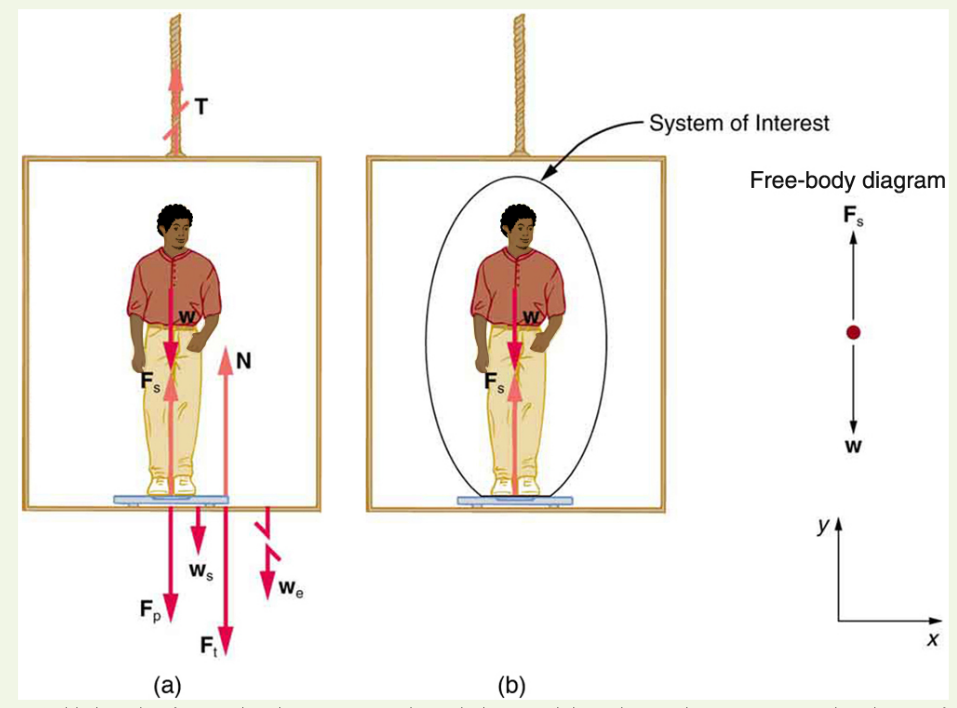
\includegraphics[width=0.4\textwidth]{elevator.png}
\caption{\label{fig:elev} A person of weight $\vec{w}$ stands on a scale in an elevator.}
\end{figure}
\end{enumerate}

\end{document}
